\section{Clustering}
\smallskip \hrule height 2pt \smallskip

\begin{itemize}
	\item Unsupervised learning: detect patterns in unlabeled data. 
		Sometmes labels are too expensive, unclear, etc. to get them.
		Examples:
		\begin{itemize}
			\item group e-mails or search results
			\item find categories of customers
			\item detect anomalous program execuations
		\end{itemize}
	\item Useful when you don't know what you are looking for. 
	\item Requires a definition of "similar".  One option: small (squared) euclidean distance. 
	\item You can label then use the clusters, or use the clusters for the next level of anlaysis.
\end{itemize}

\subsection{K-Means}
An iterative clustering algorithm.  \hfill \\
Pick K random points as cluster means: $c^1, \dots, c^k$.  \hfill \\
Alternate:
\begin{itemize}
	\item Assign each example $x^i$ to the mean $c^i$ that is closest to it
	\item Set each mean $c^i$ to the average of its assigned points. 
\end{itemize}
Stop when no points' assignments change. \hfill \\

Minimizing a loss that is a function of the points, assignments, and means:
$$ L( \{ x*i \},  \{ a*j \},   \{ c*k \}) = \sum_i dist(x^i, c^{a^i}$$
Coordinate gradient descent on L.  \hfill \\

More formally: 
\begin{itemize}
	\item Data: $\{ x^j | j = 1 \dots n \}$
	\item For $ t = 1 \dots T$:  (or stop if assignments don't change): \hfill \\
		Fix means ($c$) while you change the assignments ($a$): \hfill \\
		\begin{itemize}
			
			\item for $ j = 1 \dots n$: (recompute cluster assignments):
				$$ a^j = \argmin_i dist(x^j, c^i)  $$ 
		\end{itemize}
	\item fix assignments ($a$) while you change the means ($c$): \hfill \\
		for $j = 1 \dots k$: (recompute cluster centers)
		$$ c^j = \frac{1}{|\{ i | a^i = j \}|}  \sum_{\{ i | a^i = j \}} x^i$$
\end{itemize}
Note:  the point y with minimum squared Euclidean distance to a set of points {x} is their mean

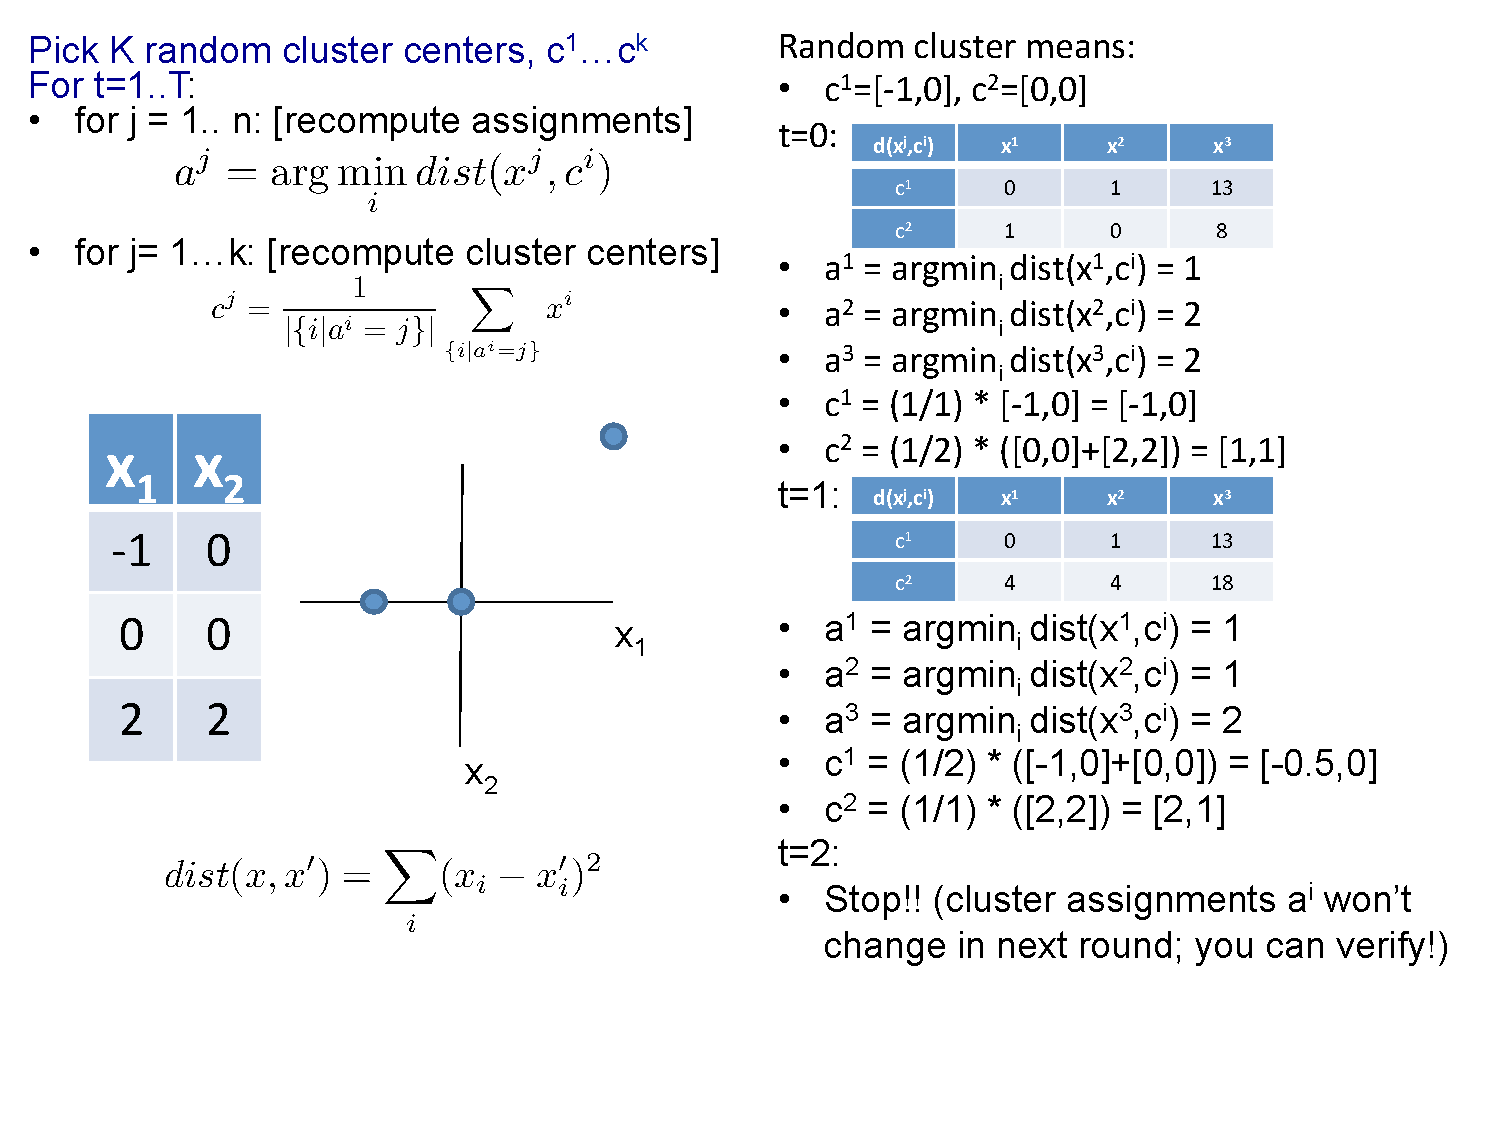
\includegraphics[width=3.3in]{figures/kmeans_algorithm_example.pdf}

\subsection{K-Means gets stuck in local optima.}

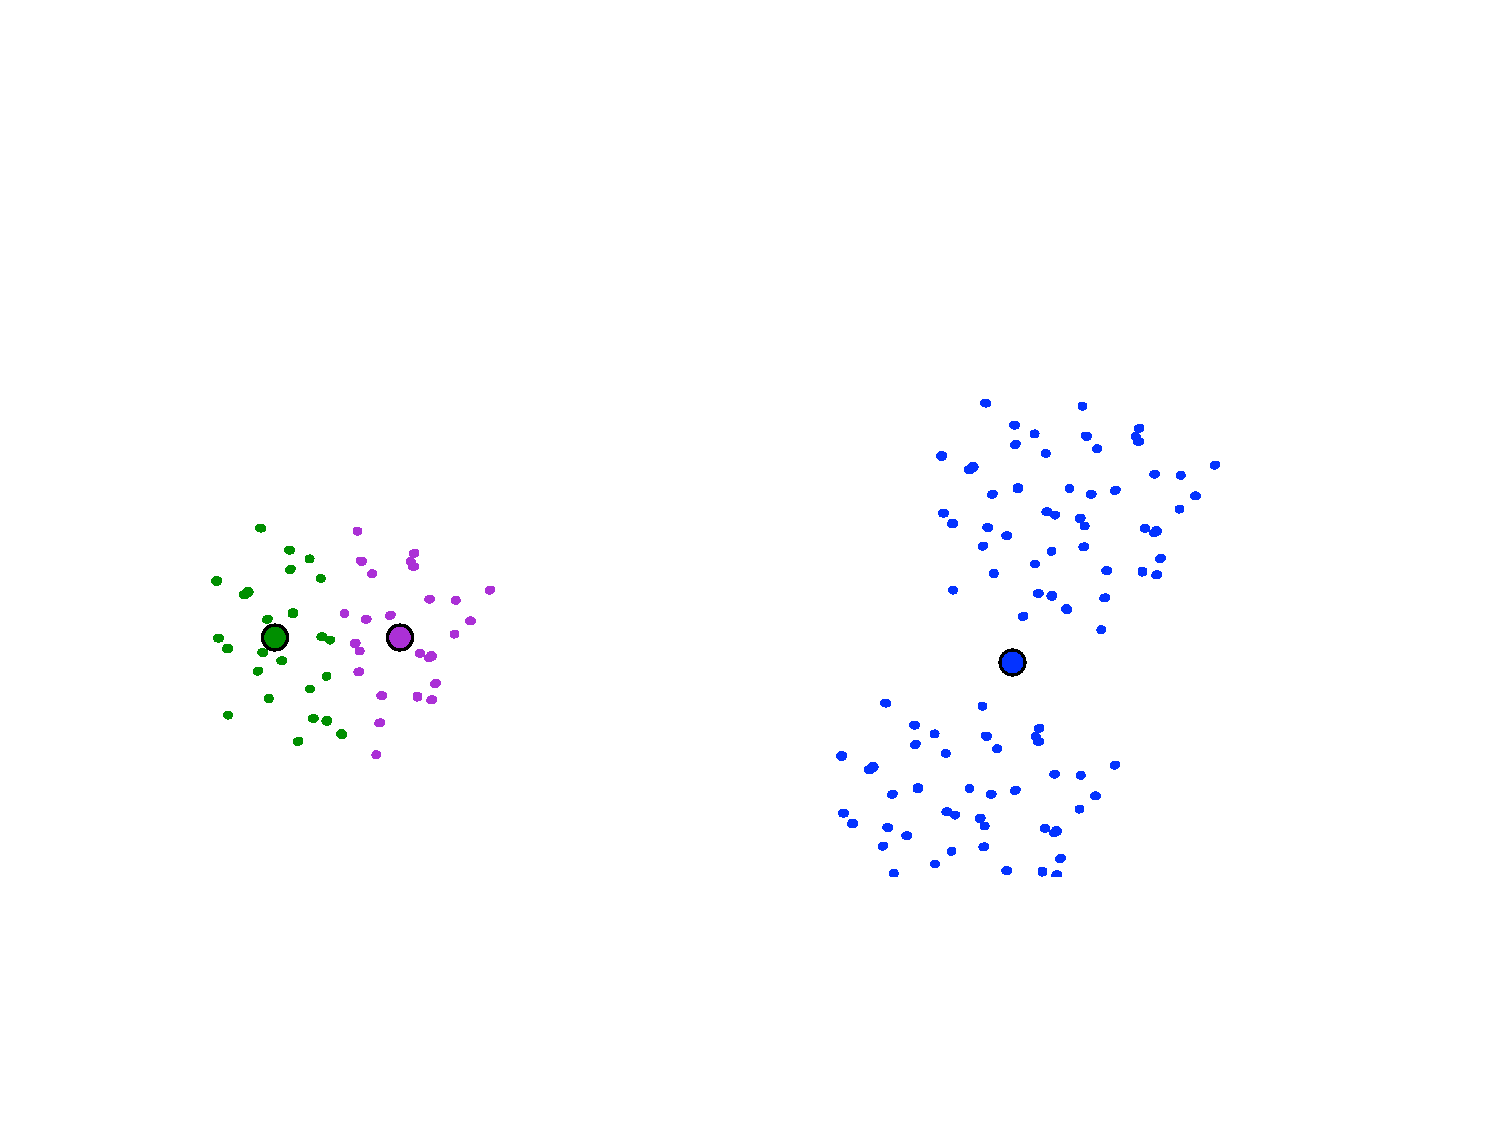
\includegraphics[width=1.8in]{figures/k-means_gets_stuck.pdf}
